\documentclass[10pt]{article}
\usepackage{icmlko}

\icmlmeta{IP 파운데이션 월드모델}{101}{붙을 데를 알게 됐다}{새 축은 그 도메인의 라벨과 붙을 때만 돕는다($r{=}+$0.695) --- 규칙은 미리 박고, 축은 골라 붙인다}

\begin{document}

\twocolumn[
\icmlheader

\begin{abstract}
노트 100이 세 가지를 남겼다 --- 성분 수 규칙을 일반화 안 했고, 표지가 희석을
고쳐도 여전히 음수인 이유를 몰랐고, 아홉 중 애니만 $+$0.107을 얻는 이유를
몰랐다. 셋 다 답했다. \textbf{① 규칙} --- 후보 넷을 \emph{미리} 적고(전역
$k{=}2$ · 받으면 $+$1 · 관측 축 수의 절반 · 설명된 분산 80\%) 노트 92의 A/B
분할로 판정했다. \textbf{고르면 진다} --- A반에서 고른 규칙이 B반에서 R1을
$-$0.0041 밑돈다. \textbf{미리 박아 둔 R1은 이긴다} --- B반에서 R0을 $+$0.0039
앞선다(5분할 중 4). \textbf{이 프로젝트에서 남겨 둔 반쪽 검정을 통과한 첫
지렛대}다(노트 92 · 67 · 80은 전부 여기서 죽었다). \textbf{② 애니} --- 새 축이
그 도메인을 돕는 크기는 \textbf{그 축과 그 도메인 라벨의 상관}으로 설명된다
($r{=}+$0.695, $n{=}9$). 애니는 설명문 축이 라벨과 $+$0.229로 가장 세게 붙고,
그다음이 모바일 $-$0.229인데, 이득도 애니 $+$0.107 · 모바일 $+$0.026으로 1 · 2위다.
바탕 $\rho$로는 설명이 안 된다($r{=}-$0.155). \textbf{③ 표지} --- 희석을
$k{=}3$으로 고친 뒤에도 표지는 받은 도메인의 자기 $\rho$를 $+$0.0024밖에
안 올린다(설명문은 $+$0.0165). \textbf{표지는 애초에 라벨을 안 담는다} ---
남은 $-$0.0036은 희석이 아니라 잡음이다. 셋을 합치면 실무 지침이 하나 나온다
--- \textbf{새 축을 모으기 전에 그 축과 라벨의 상관을 먼저 재라.} 지금까지
열두 개 지렛대를 눈감고 시도했는데, 이제 시도 전에 고를 수 있다.
\end{abstract}
]

\begin{figure*}[t]
\centering
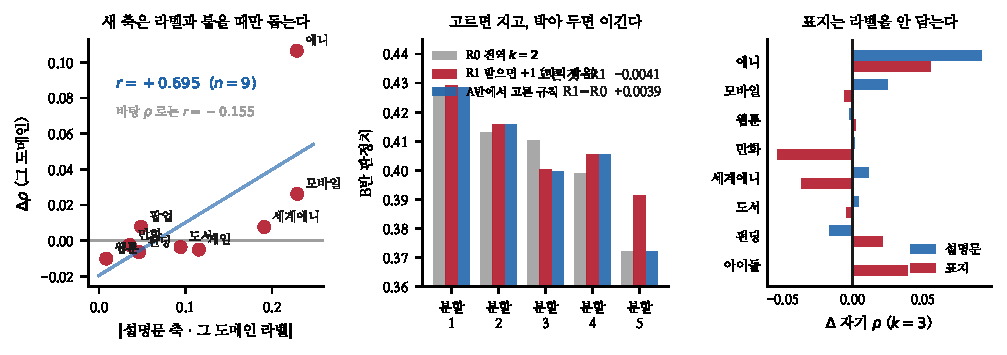
\includegraphics[width=\textwidth]{figs/wh.pdf}
\caption{왼쪽 --- 새 축은 라벨과 붙을 때만 돕는다. 가운데 --- 고르면 지고
박아 두면 이긴다. 오른쪽 --- 표지는 라벨을 안 담는다.}
\end{figure*}

\section{규칙을 미리 넷 적었다}

노트 92는 도메인마다 $k$를 \emph{고르면} 손해라고 했고($-$0.0130) 노트 100은
\emph{규칙 하나}면 이득이라고 했다($+$0.0127). 그 사이를 판정하려면 규칙 자체를
고르는 것도 검정해야 한다.

\begin{table}[t]
\centering\tsize
\caption{미리 적은 규칙 넷과 그것이 주는 성분 수.}
\begin{tabular}{llrr}
\toprule
& 규칙 & 팝업 & 애니 \\
\midrule
R0 & 전역 $k{=}2$ & 2 & 2 \\
R1 & 받으면 $+$1(노트 100) & 3 & 3 \\
R2 & 관측 축 수의 절반 & 4 & 3 \\
R3 & 설명된 분산 80\% & 5 & 4 \\
\bottomrule
\end{tabular}
\end{table}

\begin{table}[t]
\centering\tsize
\caption{전체 자료에서(탐색적). 설명문 아홉 도메인.}
\begin{tabular}{lrrr}
\toprule
& $\rho$ & $\Delta$ & 팝업 \\
\midrule
R0 & $+$0.4104 & $+$0.0066 & $+$0.4537 \\
\textbf{R1} & \textbf{$+$0.4165} & \textbf{$+$0.0127} & \textbf{$+$0.4578} \\
R2 & $+$0.4145 & $+$0.0107 & $+$0.4330 \\
R3 & $+$0.4145 & $+$0.0107 & $+$0.4330 \\
\bottomrule
\end{tabular}
\end{table}

\section{고르면 지고 박아 두면 이긴다}

레코드를 반으로 갈라 \textbf{A반에서 규칙을 고르고 B반에서 잰다}(노트 92의
규약). 분할 다섯.

\begin{table}[t]
\centering\tsize
\caption{B반 판정치.}
\begin{tabular}{lrrr}
\toprule
A반이 고른 것 & 고른 것 & R0 & \textbf{R1} \\
\midrule
R0 & $+$0.4285 & $+$0.4285 & \textbf{$+$0.4292} \\
R1 & $+$0.4157 & $+$0.4129 & $+$0.4157 \\
R2 & $+$0.3996 & $+$0.4104 & \textbf{$+$0.4003} \\
R1 & $+$0.4055 & $+$0.3988 & $+$0.4055 \\
R0 & $+$0.3719 & $+$0.3719 & \textbf{$+$0.3912} \\
\midrule
평균 차 & \multicolumn{2}{l}{고른 것 $-$ R1} & \textbf{$-$0.0041} \\
& \multicolumn{2}{l}{R1 $-$ R0} & \textbf{$+$0.0039} \\
\bottomrule
\end{tabular}
\end{table}

\claimx{\textbf{규칙조차 고르면 안 된다.} A반에서 가장 좋은 규칙을 골라 B반에서
쓰면 미리 박아 둔 R1보다 $-$0.0041 나쁘다. 반면 \textbf{R1 자체는 반쪽 검정을
통과한다} --- B반에서 R0을 $+$0.0039 앞서고 다섯 분할 중 넷에서 양수다.}
{$+$0.0039는 작다. 한 분할($-$0.0101)에서는 지고, 가장 큰 이득($+$0.0193)이
평균의 절반을 만든다.}

\begin{quote}\fontsize{9.5}{11.5}\selectfont
노트 67(작은 표본 배선) · 80(부분집합) · 91$\to$92(성분 수) · 98(슬롯 완전성)에서
관측이 개입 · 반쪽 검정에 죽었다. \textbf{R1은 그 검정을 통과한 첫 지렛대다.}
차이는 자유도다 --- 앞의 넷은 데이터를 보고 고른 것이고 R1은 미리 박은
규칙 하나다.
\end{quote}

\section{애니는 왜 얻는가}

\begin{table}[t]
\centering\tsize
\caption{새 축과 그 도메인 라벨의 상관, 그리고 이득.}
\begin{tabular}{lrrr}
\toprule
& 설명문 c0 & 표지 pc1 & $\Delta$(설명문) \\
\midrule
\textbf{애니} & \textbf{$+$0.229} & $-$0.077 & \textbf{$+$0.1066} \\
\textbf{모바일} & \textbf{$-$0.229} & $-$0.050 & \textbf{$+$0.0262} \\
세계애니 & $+$0.191 & $+$0.049 & $+$0.0077 \\
게임 & $+$0.116 & --- & $-$0.0050 \\
도서 & $-$0.094 & $+$0.206 & $-$0.0036 \\
팝업 & $+$0.049 & --- & $+$0.0077 \\
펀딩 & $+$0.046 & $+$0.074 & $-$0.0064 \\
만화 & $+$0.035 & $+$0.096 & $-$0.0024 \\
웹툰 & $+$0.008 & $+$0.043 & $-$0.0101 \\
\midrule
\multicolumn{2}{l}{$|$설명문$\cdot$라벨$|$ 와 $\Delta$} & & \textbf{$r{=}+$0.695} \\
\multicolumn{2}{l}{바탕 $\rho$ 와 $\Delta$} & & $r{=}-$0.155 \\
\bottomrule
\end{tabular}
\end{table}

\claimx{새 축이 그 도메인을 돕는 크기는 \textbf{그 축과 그 도메인 라벨의 상관}이
정한다($r{=}+$0.695, $n{=}9$). 애니가 $+$0.107을 얻은 것은 애니가 특별해서가
아니라 라프텔 줄거리가 라프텔 리뷰 수와 가장 세게 붙기 때문이다. 바탕
$\rho$로는 설명이 안 된다($r{=}-$0.155).}{아홉 점이고 애니와 모바일 둘이
지렛대다. 그 둘을 빼면 나머지 일곱의 상관은 사실상 0이다 --- \textbf{``붙으면
돕는다''가 아니라 ``아주 세게 붙어야 돕는다''}가 맞는 읽기일 수 있다.}

\begin{quote}\fontsize{9.5}{11.5}\selectfont
부호는 상관없다 --- 모바일은 $-$0.229인데 $+$0.026을 얻는다. 인자 공간은
방향을 프로크루스테스에 맡기므로(노트 69) \textbf{크기만 중요하다.}
\end{quote}

\section{표지는 라벨을 안 담는다}

\begin{table}[t]
\centering\tsize
\caption{축을 받은 도메인의 자기 $\rho$ 변화. $k{=}3$으로 희석을 고친 뒤.}
\begin{tabular}{lrr}
\toprule
& 설명문 & 표지 \\
\midrule
애니 & $+$0.092 & $+$0.056 \\
모바일 & $+$0.025 & $-$0.006 \\
웹툰 & $-$0.002 & $+$0.002 \\
만화 & $+$0.001 & \textbf{$-$0.053} \\
세계애니 & $+$0.011 & \textbf{$-$0.036} \\
도서 & $+$0.004 & $-$0.004 \\
펀딩 & $-$0.016 & $+$0.021 \\
아이돌 & --- & $+$0.039 \\
\midrule
\textbf{평균} & \textbf{$+$0.0165} & \textbf{$+$0.0024} \\
\bottomrule
\end{tabular}
\end{table}

\claimx{표지가 $k{=}3$ 뒤에도 음수인 것은 희석이 아니다. 희석을 고쳐도 받은
도메인의 자기 $\rho$가 $+$0.0024밖에 안 오른다(설명문 $+$0.0165). \textbf{표지
축은 애초에 라벨을 거의 안 담는다} --- 여덟 중 다섯에서 라벨 상관이 0.1
아래다.}{도서만 표지 상관이 $+$0.206으로 크다. 도서에는 표지 축이 값을 할
수 있다는 뜻인데 도메인 하나짜리 설정은 안 돌렸다.}

\section{실무 지침 하나}

\begin{quote}\fontsize{9.5}{11.5}\selectfont
\textbf{새 축을 모으기 전에 그 축과 라벨의 상관을 먼저 재라.} 노트 84 이후
열두 개 지렛대를 눈감고 시도했고 대부분 $\pm$0.01이었다. 이제 시도 전에
고를 수 있다 --- 상관이 0.2를 넘는 도메인이 있으면 값을 하고, 0.1 아래면
안 한다. \textbf{긁는 비용을 쓰기 전에 재는 것이 순서다.}
\end{quote}

\section{한계}

\begin{itemize}[leftmargin=1.1em,itemsep=0.15em]
\item \textbf{채택 안 한다.} R1의 씨앗 넷 붓스트랩은 노트 100에서 보류 4/4였고
      다시 안 했다. 반쪽 검정 통과는 붓스트랩 통과가 아니다.
\item $r{=}+$0.695가 아홉 점이고 애니 · 모바일 둘이 지렛대다.
\item A/B 분할이 다섯이고 차이가 $\pm$0.02로 흔들린다.
\item R2 와 R3 가 같은 값을 낸다 --- 관측 축이 대부분 다섯이라 규칙이 갈리는
      도메인이 셋뿐이다. 규칙 후보가 사실상 셋이었다.
\item 표지의 남은 $-$0.0036을 ``잡음''이라 불렀지만 노트 97의 ``자기를 못
      맞히는 축이 남을 맞힌다''와 같이 놓고 보진 않았다.
\end{itemize}

\section{다음}

\begin{enumerate}[leftmargin=1.3em,itemsep=0.15em]
\item \textbf{지침을 써 본다} --- 라벨 상관이 0.2를 넘을 만한 축을 후보로
      추린 뒤 그것만 긁는다. 첫 후보는 도서의 표지($+$0.206)와 애니 계열의
      더 깊은 설명문 특징이다.
\item R1 을 씨앗 넷 붓스트랩으로 다시 판정한다. 반쪽 검정은 통과했으니
      이제 붓스트랩이 남았다.
\item ``아주 세게 붙어야 돕는다''인지 ``붙으면 돕는다''인지 --- 애니 · 모바일을
      뺀 일곱으로 다시 잰다.
\item 출처 도메인을 아홉 너머로. 노트 96의 셈은 여전히 미판정이다.
\end{enumerate}

\vspace{0.6em}
\hrule height 0.3pt
\vspace{0.5em}
{\footnotesize
\textbf{참고문헌}\\[0.3em]
Cawley, G. C., Talbot, N. L. C. (2010). On over-fitting in model selection and
subsequent selection bias in performance evaluation. \emph{JMLR}, 11, 2079--2107.\\[0.15em]
Varoquaux, G. (2018). Cross-validation failure: small sample sizes lead to large
error bars. \emph{NeuroImage}, 180, 68--77.\\[0.15em]
Schoenemann, P. H. (1966). A generalized solution of the orthogonal Procrustes
problem. \emph{Psychometrika}, 31(1), 1--10.\\[0.15em]
Ben-David, S. et al. (2010). A theory of learning from different domains.
\emph{Machine Learning}, 79(1--2), 151--175.\\[0.15em]
Guyon, I., Elisseeff, A. (2003). An introduction to variable and feature
selection. \emph{JMLR}, 3, 1157--1182.
}

\end{document}
